% Computed masses, not a sample. Bin(20,1/10) and Poisson(2), k=0..8.
% Heights in probability units. Checked by direct evaluation of the two formulas.
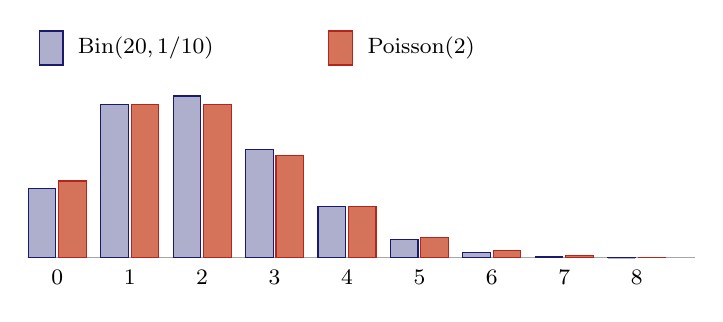
\begin{tikzpicture}[x=0.92cm,y=7.2cm,line cap=round]
  \draw[black!35] (0,0)--(9.2,0);
  \foreach \k/\b/\p in {0/0.12158/0.13534,1/0.27017/0.27067,2/0.28518/0.27067,3/0.19012/0.18045,4/0.08978/0.09022,5/0.03192/0.03609,6/0.00887/0.01203,7/0.00197/0.00344,8/0.00036/0.00086}{
    \draw[fill=MidnightBlue!35,draw=MidnightBlue] (\k,\b) rectangle (\k+0.38,0);
    \draw[fill=BrickRed!55,draw=BrickRed] (\k+0.42,0) rectangle (\k+0.80,\p);
    \node[font=\footnotesize] at (\k+0.4,-0.035) {$\k$};
  }
  \draw[fill=MidnightBlue!35,draw=MidnightBlue] (0.15,0.34) rectangle (0.48,0.40);
  \node[font=\footnotesize,anchor=west] at (0.55,0.37) {$\mathrm{Bin}(20,1/10)$};
  \draw[fill=BrickRed!55,draw=BrickRed] (4.15,0.34) rectangle (4.48,0.40);
  \node[font=\footnotesize,anchor=west] at (4.55,0.37) {Poisson$(2)$};
\end{tikzpicture}
